\documentclass[10pt,letterpaper]{article}
\usepackage[left=1.8cm, right=1.8cm, top=1cm]{geometry}
\usepackage[utf8]{inputenc}
\usepackage[T1]{fontenc}
\usepackage[spanish]{babel}
\usepackage{amsmath}
\usepackage{amsfonts}
\usepackage{amssymb}
\usepackage{graphicx}
\usepackage{subfigure}
\usepackage{steinmetz}
\usepackage{float}
%\usepackage{circuitikz}

\author{Clase Práctica $\#$4}
\title{Electrónica I}
\date{Capacitores e inductores. Circuitos en estado transitorio.\\
Análisis de circuitos en corriente alterna.}

\renewcommand{\sin}{\sen}
\begin{document}
	\maketitle
	
Bibliografía: Análisis de circuitos en ingeniería. Hayt \textit{et al.} 8va ed. Capítulos 7, 8 y 10.
\\
 
 1- El interruptor del circuito en la figura ha estado cerrado durante un tiempo ridículamente largo hasta abrirse de manera repentina en $t = 0$. 
 
 a) Obtenga expresiones para $i_L$ y $v$ en el circuito de la figura que sean válidas para todo $t \geq 0$. 
 
 b) Calcule $i_L(t)$ y $v(t)$ en el instante inmediatamente anterior a la apertura del interruptor, en el instante inmediatamente posterior a la apertura del interruptor, y en el $t = 470 \: \mu s$.
 
 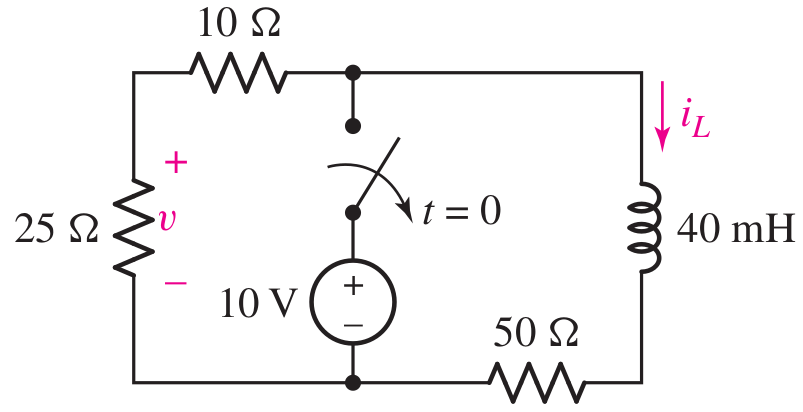
\includegraphics[scale=0.3]{c1}
 \\
 
 2- Es seguro suponer que un interruptor dibujado en el circuito de la figura ha estado cerrado durante un tiempo tan largo que cualquier transitorio que podría haber surgido desde la primera vez que se conectó la fuente de tensión ha desaparecido.
 
 a) Determine la constante de tiempo del circuito. 
 
 b) Calcule la tensión $v(t)$ en $t =\tau$, $2\tau$ y $5 \tau$.

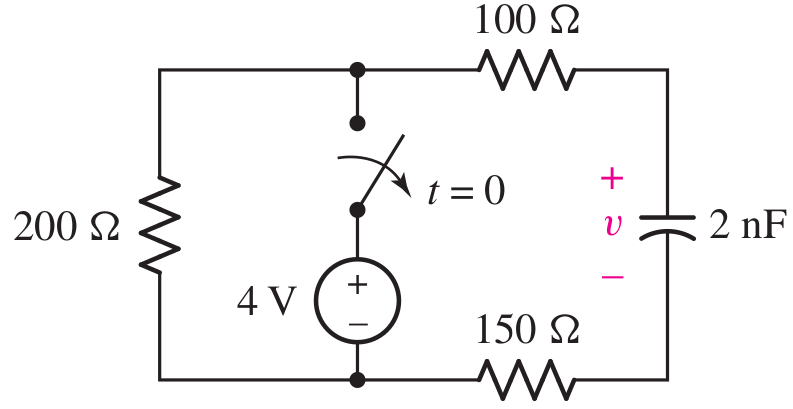
\includegraphics[scale=0.3]{c2}

3- Muestre en el circuito de la figura que para una fuente senoidal la relación entre los fasores de voltaje y corriente en el inductor es $\mathrm{j}2\pi fL$ y en el capacitor es $\dfrac{-\mathrm{j}}{2\pi fC}$.

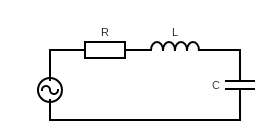
\includegraphics[scale=0.61]{c3_1}

4- Diga el fasor o la expresión temporal según corresponda: \\

a) $i_1(t)=12\sin(400t+110^{\circ}) \: [\mathrm{A}]$ \\

b) $i_2(t)=-7\sen(200t)- 3\cos(200t - 30^{\circ}) \: [\mathrm{A}]$ \\

c) $\mathrm{\textbf{V}}_1 = 70 \phase{30^{\circ}} \: [\mathrm{V}] $ \\

d) $\mathrm{\textbf{V}}_2 =-60+\mathrm{j}40 \: [\mathrm{V}] $ \\

5- En el circuito de la figura:

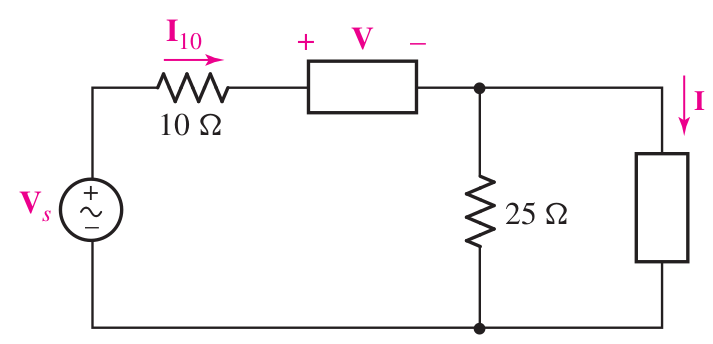
\includegraphics[scale=0.4]{c5_1}

a) Si $\textbf{I}_{10}=2\phase{42^{\circ}} \: \mathrm{mA}$ y $\textbf{V}=40\phase{132^{\circ}} \: \mathrm{mV}$, ¿cuál es probablemente el tipo de elemento conectado a la derecha de la resistencia de 10 $\Omega$? Calcule su valor suponiendo que la fuente de tensión opera a una frecuencia de 1 000 rad/s.


b) Si $\textbf{I}_{10}=4\phase{35^{\circ}} \: \mathrm{A}$, $\textbf{V}=10\phase{35^{\circ}} \: \mathrm{V}$ e $\textbf{I}=2\phase{35^{\circ}} \: \mathrm{A}$, diga que tipo de elemento corresponde a la tensión $\textbf{V}$ y su valor. Además, determine $\textbf{V}_s$.
\\

6- Utilice las técnicas de análisis fasorial para obtener expresiones para las dos corrientes de malla $i_1$ e $i_2$ como se muestra en la figura.

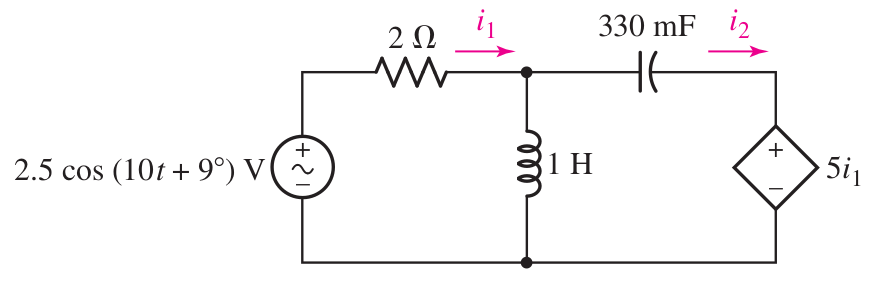
\includegraphics[scale=0.4]{c6}

%3- Obtenga expresiones tanto para $i_1(t)$ como para $i_L(t)$ como están marcados en la figura y que sean válidas para $t > 0$.
%
%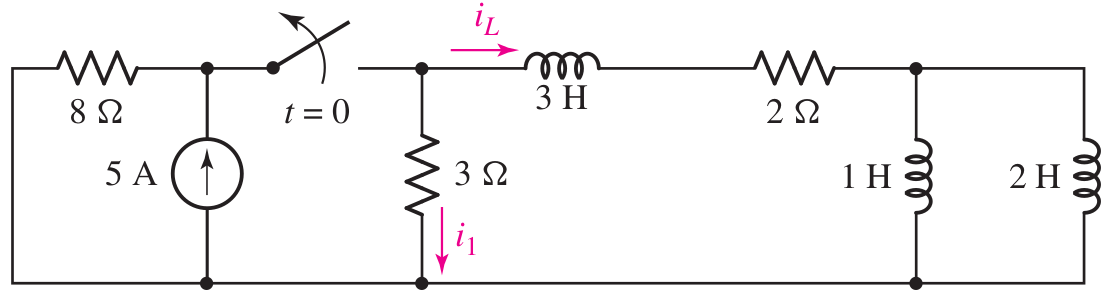
\includegraphics[scale=0.3]{c3}
%
%\pagebreak
%
%4- Seleccione valores para las resistencias $R_0$ y $R_1$ en el circuito de la figura de manera que $v_C(0.65) = 5.22 \mathrm{V}$ y $v_C(2.21) = 1 \mathrm{V}$.
%
%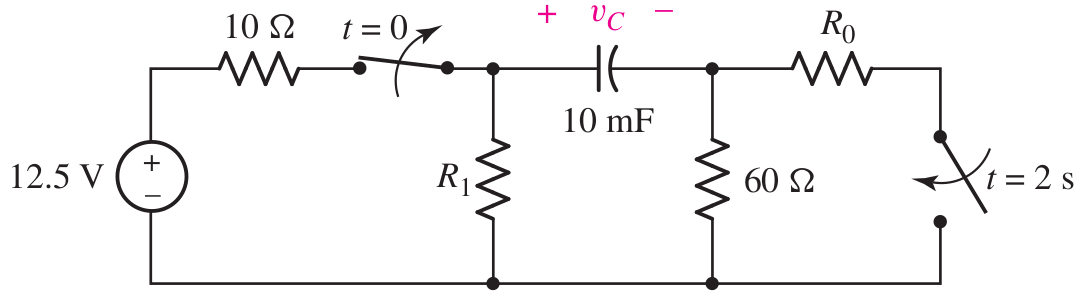
\includegraphics[scale=0.3]{c4}
%\\
%
%5- Obtenga las expresiones para la corriente $i(t)$ y la tensión $v(t)$ indicados en el circuito de la figura que sean válidas para todo $t > 0$.
%
%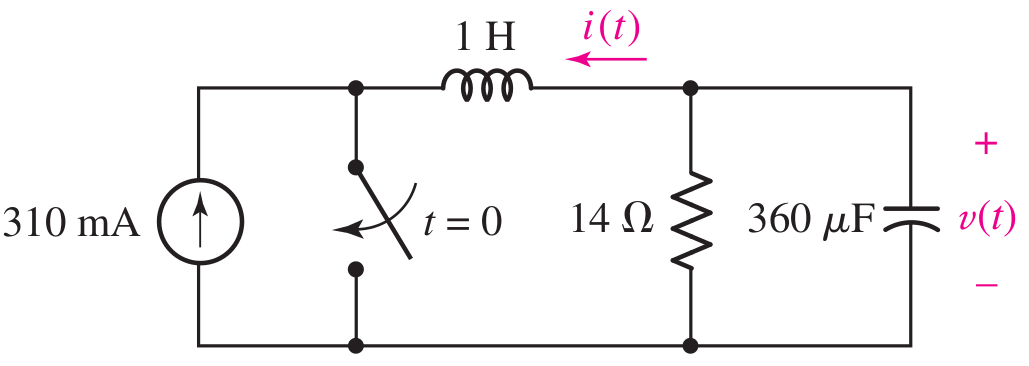
\includegraphics[scale=0.3]{c5}
\end{document}